\section{Mean field and critical behavior}

\begin{frame}{Coarse graining by block densities}
  \bookref{Chapter 3, Sections 1--2}
  \small
  Given an ordered partition
  \[
    \mathcal P=(X_1,\ldots,X_k),
    \qquad X=X_1\sqcup\cdots\sqcup X_k,
  \]
  the \emph{block profile} is the coarse tuple
  \[
    \operatorname{prof}_{\mathcal P}(S)=(\alpha,\rho),
    \quad
    \alpha_i=\frac{|X_i|}{|X|},
    \quad
    \rho_{ij}=\frac{|R\cap(X_i\times X_j)|}{|X_i||X_j|}.
  \]

  For fixed counts $m_{ij}=|R\cap(X_i\times X_j)|$, the labeled degeneracy is
  \[
    \prod_{i,j}\binom{|X_i||X_j|}{m_{ij}}.
  \]

  Using Stirling's approximation with
  $h(u)=-u\log u-(1-u)\log(1-u)$ gives the entropy density
  \[
    \mathcal S_k(\alpha,\rho)
      =\sum_{i,j}\alpha_i\alpha_j h(\rho_{ij}).
  \]
\end{frame}

\begin{frame}{Variational free energy}
  \bookref{Chapter 3, Sections 1--3}
  If $E(S)\approx n^2\Phi_k(\alpha,\rho)$, then profiles contribute at leading
  exponential order as
  \[
    Z(\beta)\approx
    \sum_{\text{profiles}}
    \exp\!\left[-n^2\mathcal F_\beta(\alpha,\rho)\right],
  \]
  where
  \[
    \boxed{\mathcal F_\beta
      =\beta\Phi_k(\alpha,\rho)
       -\sum_{i,j}\alpha_i\alpha_j h(\rho_{ij}).}
  \]

  \begin{columns}[T]
    \column{0.48\textwidth}
      \begin{block}{Homogeneous profile}
        All $\rho_{ij}$ coincide; block labels are macroscopically invisible.
      \end{block}
    \column{0.48\textwidth}
      \begin{block}{Differentiated profile}
        Within- and cross-block densities differ; the partition becomes
        structurally visible.
      \end{block}
  \end{columns}

  {\scriptsize Coarse degeneracy groups many exact isomorphism classes; it is an
  asymptotic replacement for, not an identity with, exact orbit multiplicity.}
\end{frame}

\begin{frame}{The contrast-sensitive two-block model}
  \bookref{Chapter 3, Section 4}
  For equal blocks, impose
  \[
    \rho_{11}=\rho_{22}=p,
    \qquad
    \rho_{12}=\rho_{21}=q.
  \]
  The refined free energy is
  \[
    \boxed{F_\beta(p,q)
      =-\frac{\beta J}{2}(p-q)^2-h(p)-h(q),
      \qquad 0<p,q<1.}
  \]

  It is invariant under block exchange $(p,q)\mapsto(q,p)$. Define
  \[
    m=\frac{p+q}{2},
    \qquad d=\frac{p-q}{2},
    \qquad \Delta=|p-q|=2|d|.
  \]

  \begin{block}{Model logic}
    Entropy favors $p=q=1/2$; the energy rewards contrast. The antisymmetric
    coordinate $d$ isolates block differentiation.
  \end{block}
\end{frame}

\begin{frame}{Exact Hessian instability}
  \bookref{Chapter 3, Section 4}
  \small
  At the symmetric point $(p,q)=(1/2,1/2)$,
  \[
    H=
    \begin{pmatrix}
      4-\beta J & \beta J\\
      \beta J & 4-\beta J
    \end{pmatrix}.
  \]

  \begin{center}
    \begin{tabular}{lcc}
      \toprule
      mode & eigenvector & eigenvalue \\
      \midrule
      mean-density & $(1,1)$ & $\lambda_{+}=4$ \\
      block-contrast & $(1,-1)$ & $\lambda_{-}=4-2\beta J$ \\
      \bottomrule
    \end{tabular}
  \end{center}

  \begin{center}
    \alert{$\displaystyle \beta_c=\frac{2}{J}$} is the exact
    loss-of-local-stability threshold in the antisymmetric mode.
  \end{center}

  \begin{alertblock}{Logical boundary}
    A negative Hessian direction proves instability, not by itself the
    existence of a nearby nonzero stationary branch.
  \end{alertblock}
\end{frame}

\begin{frame}{The fourth-order Landau jet}
  \bookref{Chapter 3, Section 5}
  \footnotesize
  Restrict to the symmetric contrast slice $m=1/2$:
  \[
    \mathcal G_{\beta,J}(d)
      =-2\beta Jd^2-h(1/2+d)-h(1/2-d).
  \]
  Its exact derivatives through order four give
  \[
    J_0^4\mathcal G(d)
      =F_0+(4-2\beta J)d^2+\frac{8}{3}d^4.
  \]

  For the quartic approximation and $\beta>\beta_c$,
  \[
    d_*^2=\frac{3}{8}(\beta J-2),
    \qquad
    \Delta\sim(\beta-\beta_c)^{1/2},
    \qquad
    D_{\mathrm{cont}}=(p-q)^2\sim(\beta-\beta_c).
  \]

  \begin{block}{Formal status}
    Lean verifies the jet and, for $|d|\le r<1/2$, the uniform bound
    \[
      |\mathcal G(d)-J_0^4\mathcal G(d)|
      \le \frac{128}{1-4r^2}|d|^6.
    \]
    The fixed-mean expansion also has a Lean proof of its $O(d^6)$ remainder
    for every $0<m<1$.
  \end{block}
\end{frame}

\begin{frame}{The exact broken minimum pair is unique}
  \bookref{Chapter 3, Section 5}
  \small
  Let $H_{\beta,J}(d)=\mathcal G_{\beta,J}'(d)$.  On $|d|<1/2$,
  \[
    H_{\beta,J}(d)=0
    \quad\Longleftrightarrow\quad
    \nabla F_\beta(1/2+d,1/2-d)=0.
  \]

  If $2<\beta J<2\log 3$, then
  \[
    H'(0)=8-4\beta J<0,
    \qquad
    H(1/4)=-\beta J+2\log 3>0.
  \]

  \begin{center}
    \begin{tikzpicture}[x=2.0cm,y=0.65cm]
      \draw[->] (-0.15,0) -- (2.25,0) node[right] {$d$};
      \fill (0,0) circle (1.2pt) node[below] {$0$};
      \fill (0.75,0) circle (1.2pt) node[below] {$t$};
      \fill (2,0) circle (1.2pt) node[below] {$1/4$};
      \node[above] at (0.75,0) {$H(t)<0$};
      \node[above] at (2,0) {$H(1/4)>0$};
      \draw[thick,draw=RelTeal] (0,0) .. controls (0.45,-0.75) and (0.9,-0.65) ..
        (1.35,0) .. controls (1.6,0.35) and (1.8,0.55) .. (2,0.7);
      \fill[fill=RelTeal] (1.35,0) circle (1.5pt) node[below] {$d_*$};
    \end{tikzpicture}
  \end{center}

  Continuity gives $d_*\in(0,1/4)$; oddness gives $-d_*$.  Strict monotonicity
  of the exact coupling map makes this pair unique, and entropy concavity plus
  positive exact slice curvature makes both points \alert{full local minima}.
\end{frame}

\begin{frame}{The exact branch has the Landau exponent}
  \bookref{Chapter 3, Section 5}
  \small
  Parameterize the positive exact branch by
  \[
    K=\beta J=\kappa(d)
      :=\frac{1}{2d}\log\!\left(\frac{1+2d}{1-2d}\right),
    \qquad 0<d<\frac12.
  \]

  The derivative remainder gives the explicit normalized estimate
  \[
    \left|\frac{\kappa(d)-2}{d^2}-\frac83\right|
      \le \frac{32d^2}{1-4d^2}.
  \]
  Therefore, as $d\downarrow0$ (equivalently $K\downarrow2$),
  \[
    \frac{d^2}{K-2}\longrightarrow\frac38,
    \qquad
    d\sim\sqrt{\frac38(K-2)}.
  \]

  \begin{alertblock}{Exact conclusion}
    The square-root law is now a theorem for the unique exact branch, not only
    the prediction of the fourth-order Landau polynomial.
  \end{alertblock}
\end{frame}

\begin{frame}{Numerical onset matches the analytic threshold}
  \bookref{Chapter 3, Section 11; Appendix B}
  \begin{columns}[T]
    \column{0.50\textwidth}
      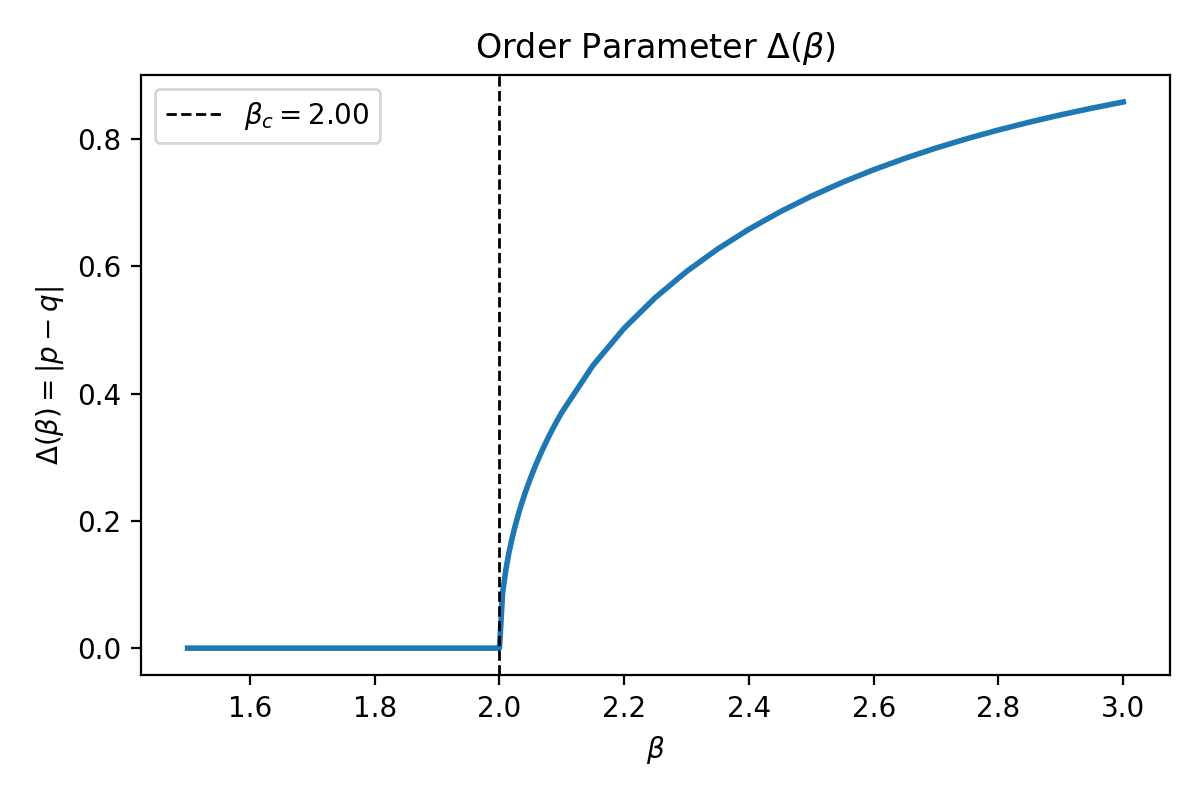
\includegraphics[width=\textwidth]{delta_vs_beta.png}
    \column{0.50\textwidth}
      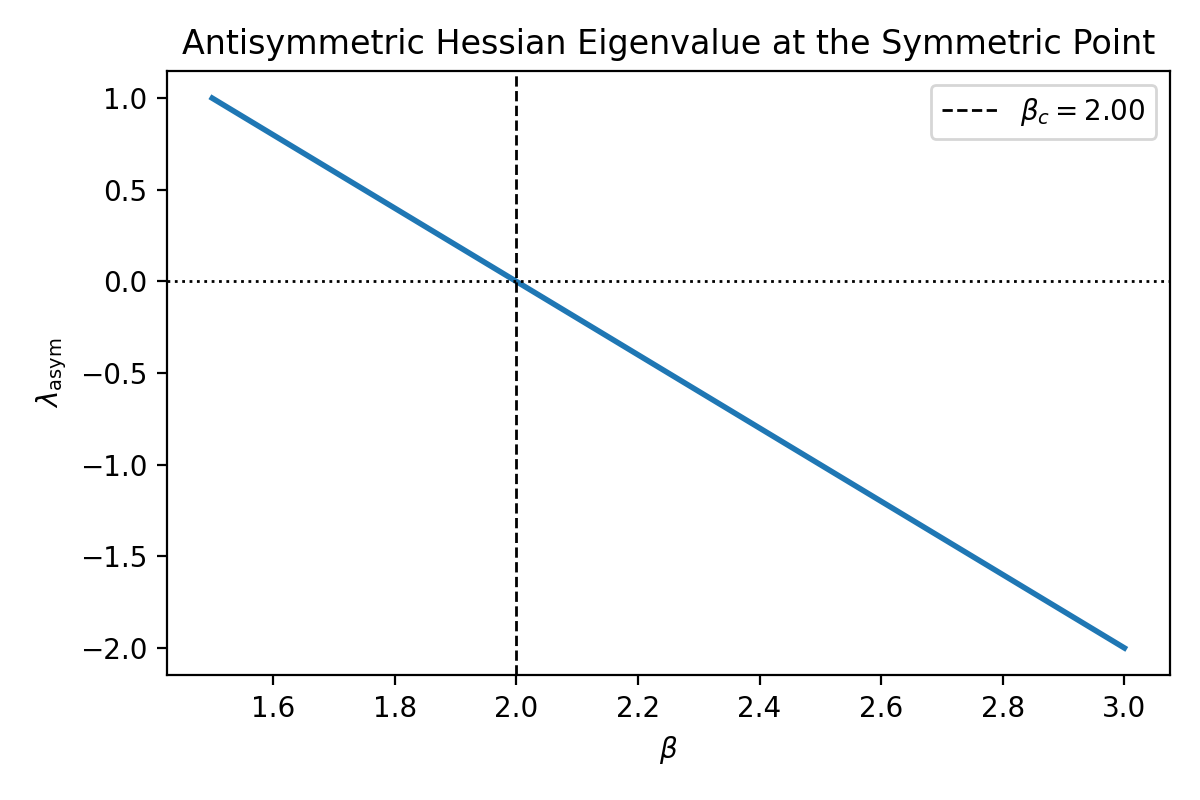
\includegraphics[width=\textwidth]{antisymmetric_eigenvalue_vs_beta.png}
  \end{columns}

  \vspace{-0.2em}
  \begin{itemize}
    \item $J=1$ predicts $\beta_c=2$.
    \item On the $0.025$ grid, the first nonzero contrast occurs at $2.025$.
    \item At that point $(p_*,q_*)=(0.595760,0.404240)$ and
      $\Delta=0.191520$.
  \end{itemize}
\end{frame}

\begin{frame}{Landau scaling is local, not global}
  \bookref{Chapter 3, Section 5; Appendix B}
  \begin{columns}[T]
    \column{0.50\textwidth}
      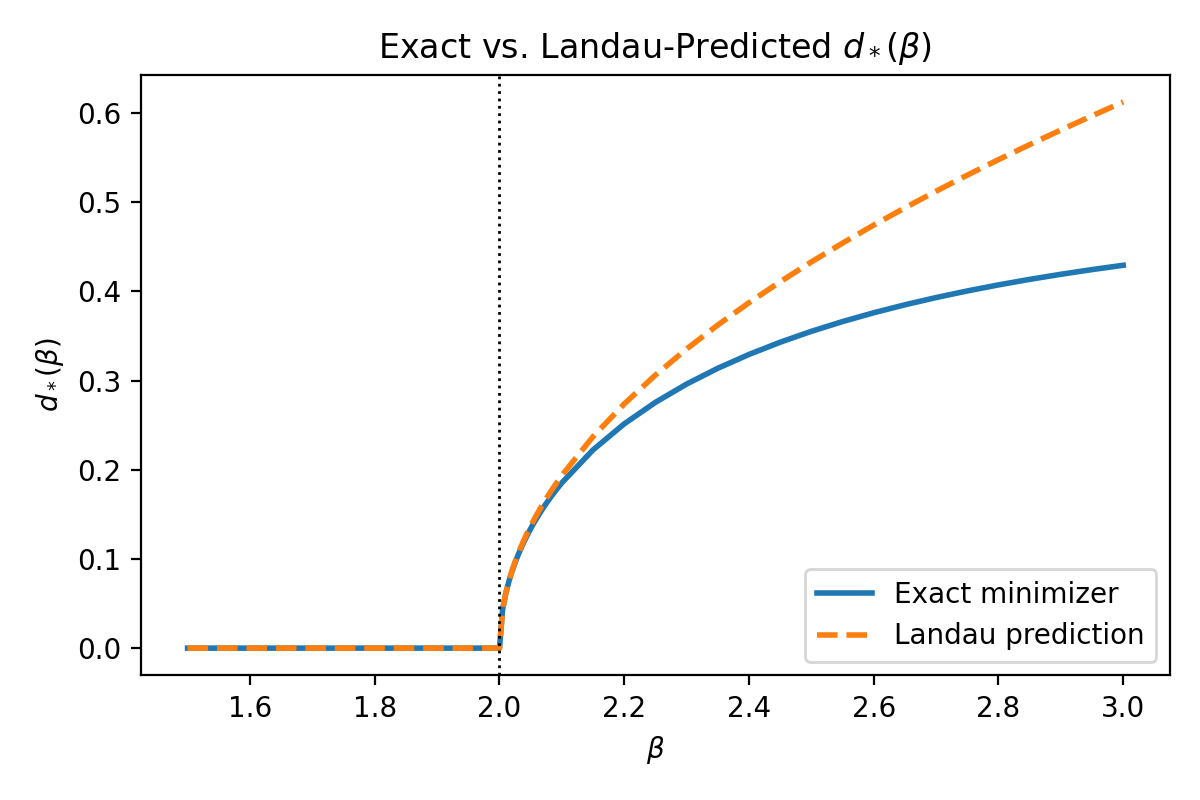
\includegraphics[width=0.84\textwidth]{d_star_exact_vs_landau.png}
      \centering{\scriptsize Exact numerical branch versus quartic prediction}
    \column{0.50\textwidth}
      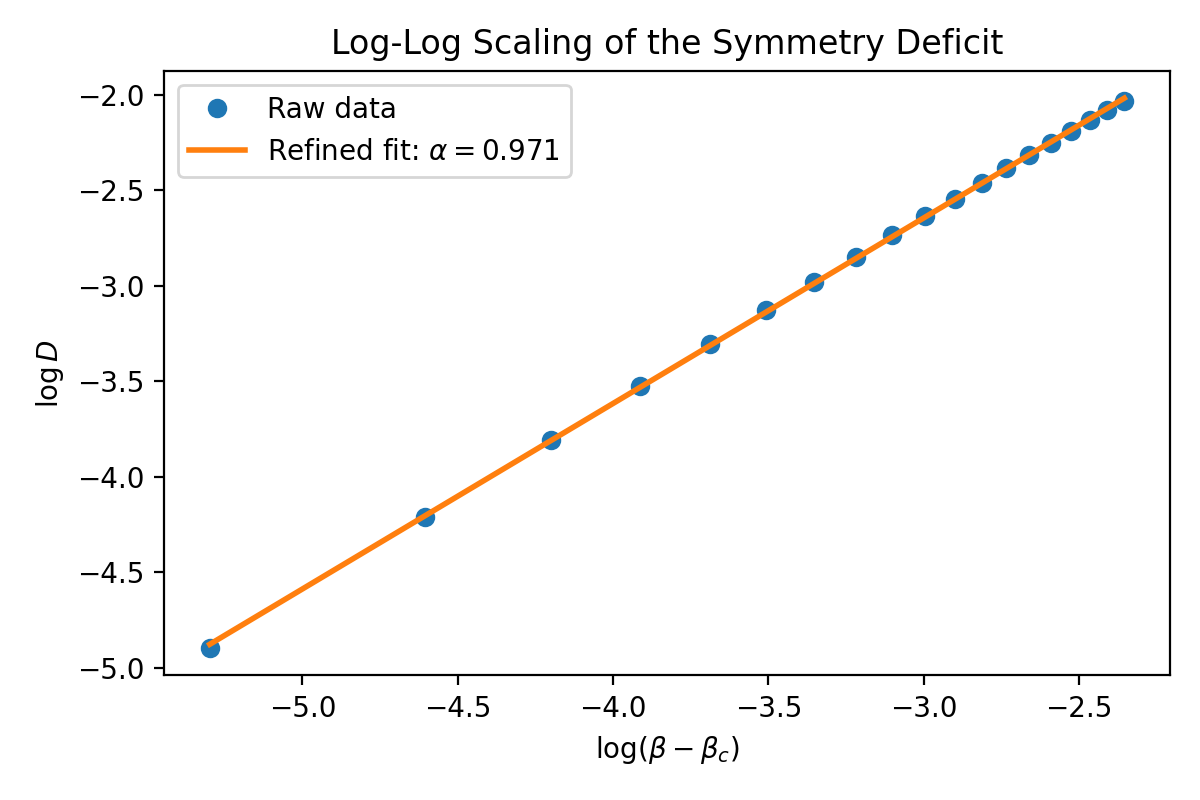
\includegraphics[width=0.84\textwidth]{scaling_symmetry_deficit.png}
      \centering{\scriptsize Near-threshold fit: slope $\alpha\approx0.971$}
  \end{columns}

  \vspace{0.1em}
  \begin{block}{Reading the evidence}
    The branch and $D_{\mathrm{cont}}\propto\beta-\beta_c$ scaling agree near
    onset. Deviations away from the critical neighborhood are expected because
    the quartic jet discards higher-order terms.
  \end{block}
\end{frame}

\begin{frame}{Residual symmetry versus contrast magnitude}
  \bookref{Chapter 3, Section 11}
  Let $\Gamma=\{e,\tau\}\cong S_2$ act by $\tau(p,q)=(q,p)$. Define
  \[
    I_\Gamma(p,q)=
    \log\frac{|\Gamma|}{|\Stab_\Gamma(p,q)|}.
  \]
  Then exactly
  \[
    I_\Gamma(p,q)=
    \begin{cases}
      0,&p=q,\\
      \log 2,&p\neq q.
    \end{cases}
    \qquad
    I_\Gamma=0\iff\Delta=0.
  \]

  \begin{columns}[T]
    \column{0.48\textwidth}
      \begin{block}{Discrete invariant $I_\Gamma$}
        Detects whether block-exchange symmetry survives.
      \end{block}
    \column{0.48\textwidth}
      \begin{block}{Continuous proxy $D_{\mathrm{cont}}$}
        $(p-q)^2$ measures how far the state lies from the fixed locus.
      \end{block}
  \end{columns}
\end{frame}

\begin{frame}{Spatial test: a two-state lattice model}
  \bookref{Appendices B--C}
  \small
  For Potts spins $s_x\in\{1,\dots,q\}$ on an $L\times L$ periodic lattice,
  \[
    E=-J\sum_{\langle x,y\rangle}\delta(s_x,s_y),
    \qquad
    D_{\mathrm{lat}}=\frac1q\sum_{i=1}^q
      \left(f_i-\frac1q\right)^2.
  \]

  \begin{columns}[T]
    \column{0.50\textwidth}
      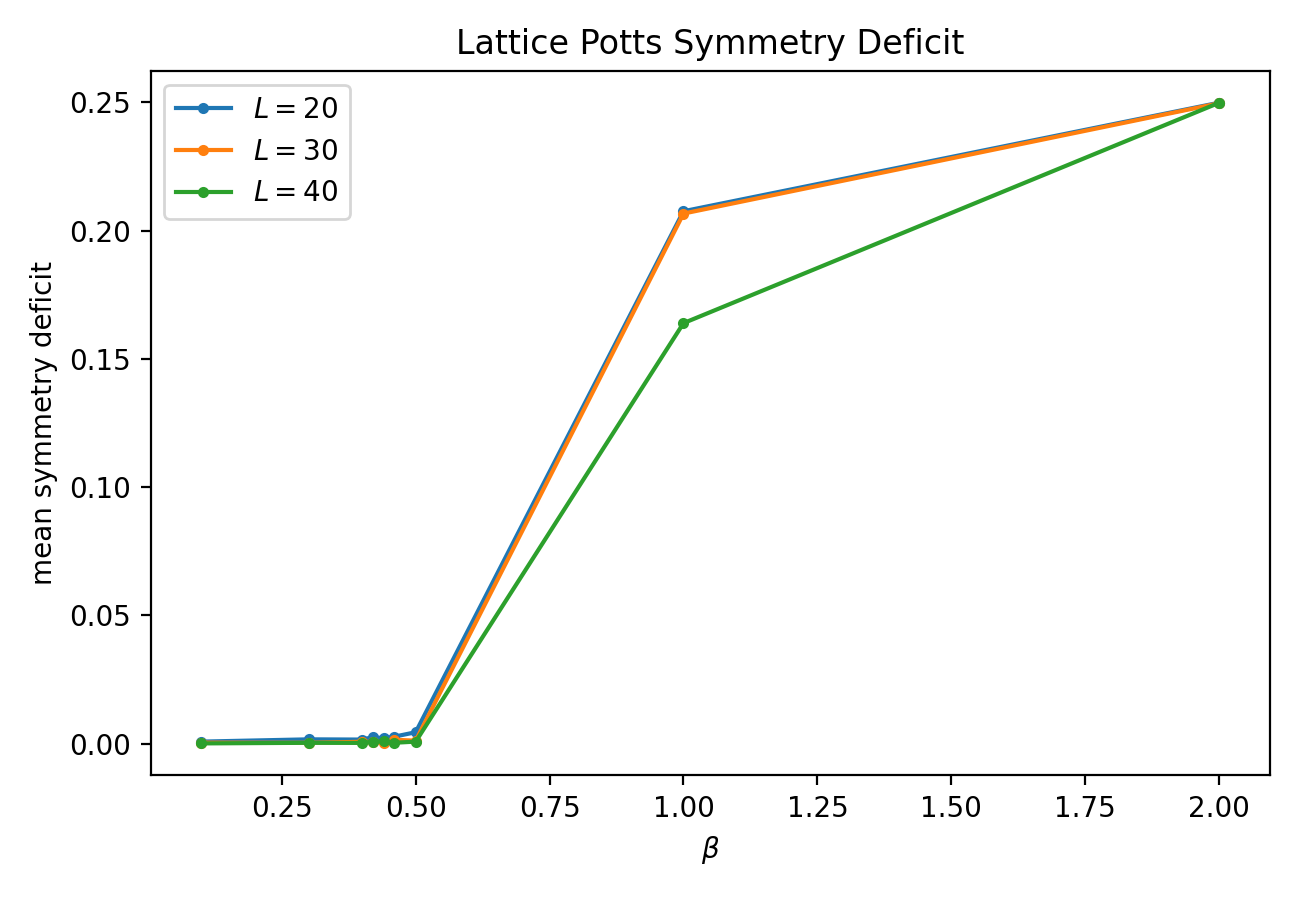
\includegraphics[width=0.88\textwidth]{lattice_symmetry_deficit.png}
    \column{0.50\textwidth}
      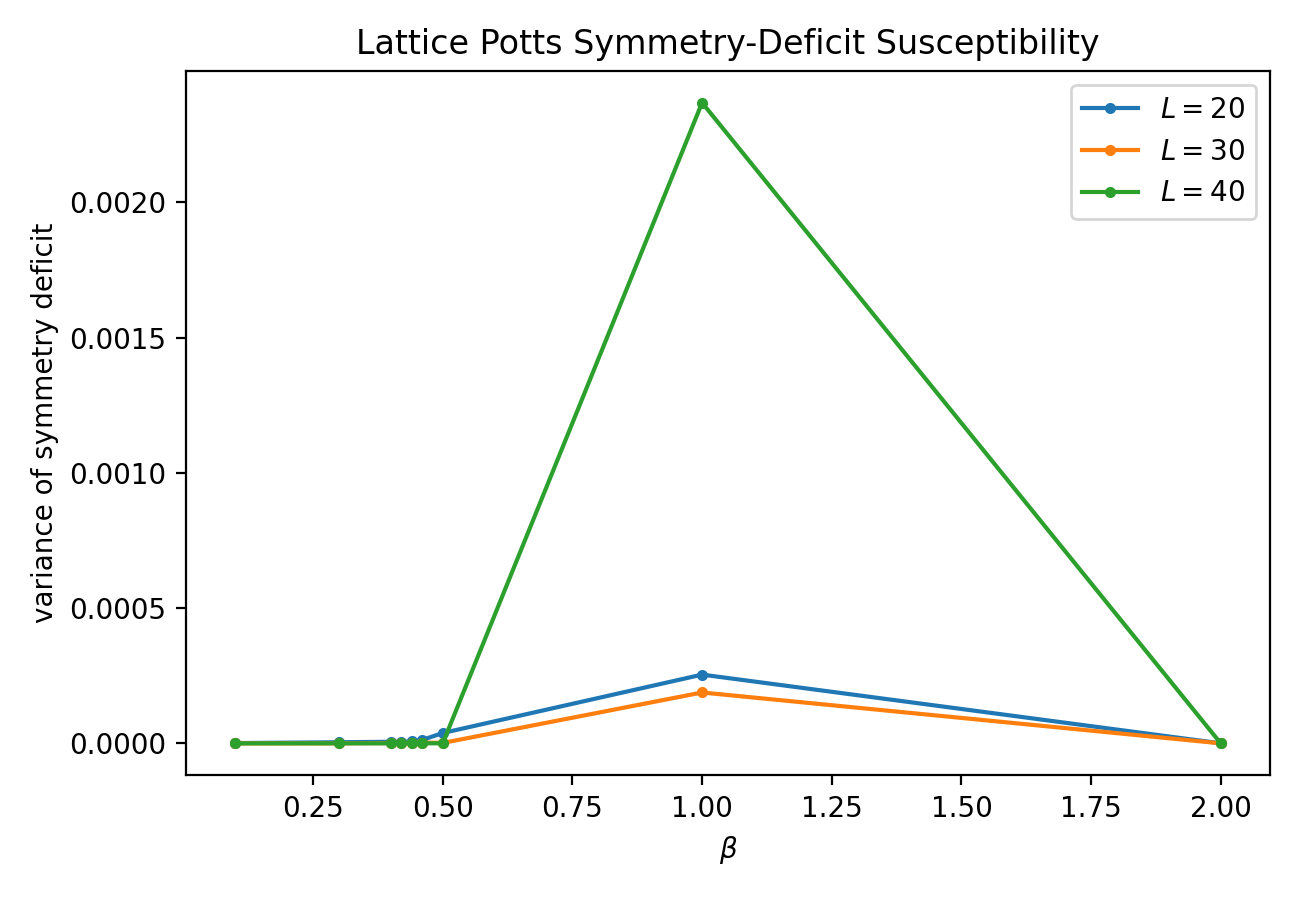
\includegraphics[width=0.88\textwidth]{lattice_susceptibility.png}
  \end{columns}

  \vspace{-0.25em}
  {\scriptsize For $L=20,30,40$, the structural observable detects ordering and
  its raw-variance peak sharpens qualitatively with size.}
\end{frame}

\begin{frame}{What the lattice data do—and do not—show}
  \bookref{Appendix C}
  \begin{columns}[T]
    \column{0.48\textwidth}
      \begin{block}{Supported}
        \begin{itemize}
          \item $D_{\mathrm{lat}}$ is small in the symmetric regime.
          \item It approaches the ordered two-state value at large $\beta$.
          \item The raw fluctuation variance shows finite-size sharpening.
        \end{itemize}
      \end{block}
    \column{0.48\textwidth}
      \begin{alertblock}{Not yet supported}
        \begin{itemize}
          \item stable pseudocritical points,
          \item reliable critical exponents,
          \item universality-class identification,
          \item superiority to standard observables.
        \end{itemize}
      \end{alertblock}
  \end{columns}

  Current raw-variance fits have poor quality and are not estimates of
  $\gamma/\nu$. If $D\sim m^2$, the structural hypothesis predicts
  $L^d\operatorname{Var}(D)\sim L^{d-4\beta_{\rm mag}/\nu}$, giving $3/2$
  rather than $7/4$ in the 2D Ising class. A joint scaling collapse is required.
\end{frame}
